\section{Pin Assignment}


During the compilation above, the Quartus Prime Compiler was free to choose any
pins on the selected FPGA to serve as inputs and outputs. However, the DE-series board
has hardwired connections between the FPGA pins and the other components on the board.
We will use two toggle switches, labeled $SW_0$ and $SW_1$, to provide the
external inputs, $x_1$ and $x_2$, to our example circuit. These switches are connected
to the FPGA pins listed in Table \ref{tab:pinassign}. We will connect the output $f$ to a
light-emitting diode $LED_0$ on your DE5a-Net board. 
The FPGA pin assignment for the LEDs can also be found in Table~\ref{tab:pinassign}.

\begin{table}[H]
\centering
\begin{tabular}{| c | c | c | c |}
\hline
Component & $SW_0$ & $SW_1$ & {\it LED}$_0$ \\
\hline
DE5a-Net & PIN$\_$AY28 & PIN$\_$AM27 & PIN$\_$T11 \\
\hline
\end{tabular}
 
\caption{DE-Series Pin Assignments}
\label{tab:pinassign}
\end{table}

\begin{figure}[H]
   \begin{center}
      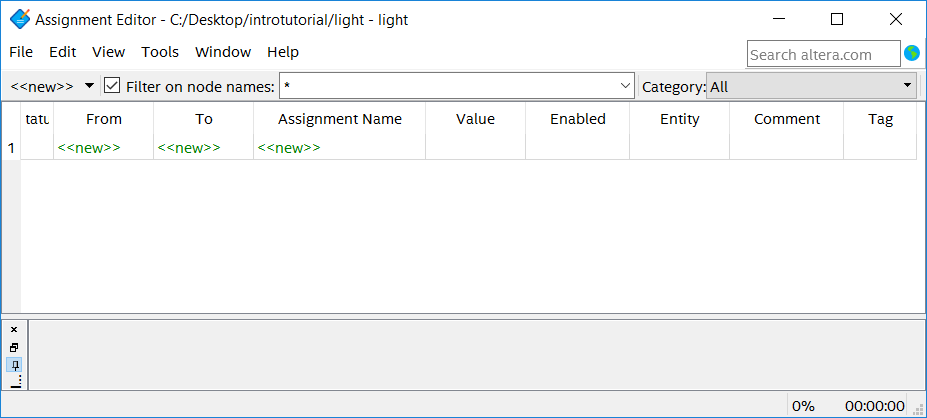
\includegraphics[scale=0.65]{figures/figure22.png}
   \caption{The Assignment Editor window.} 
	 \label{fig:22}
	 \end{center}
\end{figure}

Pin assignments are made by using the Assignment Editor. 
Select {\sf Assignments $>$ Assignment Editor} to reach the window in Figure~\ref{fig:22}
(shown here as a detached window).
In the {\sf Category} drop-down menu select {\sf All}. Click on the {\sf $<$$<$new$>$$>$} button
located near the top left corner to make a new item appear in the table. Double click the box
under the column labeled To so that the Node Finder button 
\includegraphics[scale=0.65]{figures/icon7.png}
appears. Click on the button (not the drop down arrow) to reach the window in Figure~\ref{fig:23}. Click on 
\includegraphics[scale=0.6]{figures/icon12.png} and 
\includegraphics[scale=0.6]{figures/icon15.png} to show or hide more search options.
In the {\sf Filter} drop-down menu select {\sf Pins: all}. Then click the {\sf Search} button to display
the input and output pins to be assigned: $f$, $x1$, and $x2$.
Click on $x1$ as the first pin to be assigned and click the {\sf >} button; this will enter
$x1$ in the Selected Nodes box.  Click {\sf OK}. $x1$ will now appear in the box under the column
labeled To. Alternatively, the node name can be entered directly by double-clicking the box
under the To column and typing in the node name.

Follow this by double-clicking on the box to the right of this new $x1$ entry, in the column
labeled Assignment Name. Now, the drop-down menu in Figure~\ref{fig:24} appears. Scroll down and select 
{\sf Location (Accepts wildcards)}. Instead of scrolling down the menu to find the desired item, 
you can just type the first letter of the item in the Assignment Name box. In this case the desired
item happens to be the first item beginning with L. Finally, double-click the box in the column labeled Value.
Type the pin assignment corresponding to $SW_0$ for the DE5a-Net board, as listed in Table \ref{tab:pinassign}.

Use the same procedure to assign input $x2$ and output $f$ to the appropriate pins listed in
Table \ref{tab:pinassign}. An example using a DE5a-Net board is shown in Figure~\ref{fig:25}.
To save the assignments made, choose {\sf File $>$ Save}. You can also simply close 
the Assignment Editor window, in which case a pop-up box will ask if you want to save
the changes to assignments; click {\sf Yes}.
Recompile the circuit, so that it will be compiled with the correct pin assignments.


\begin{figure}[H]
   \begin{center}
      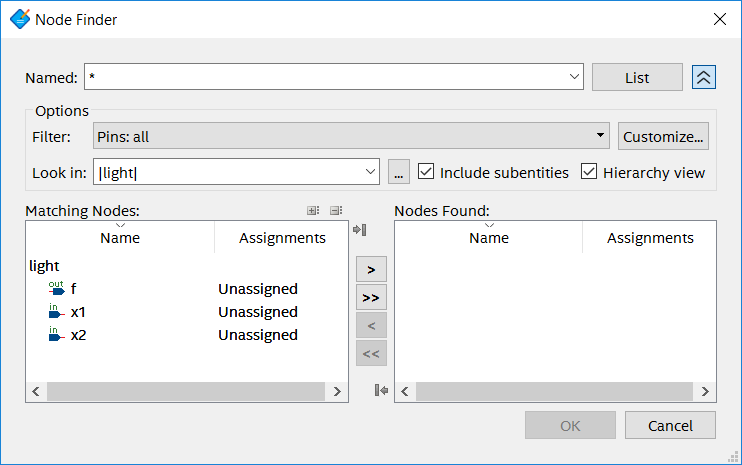
\includegraphics[scale=0.65]{figures/figure23.png}
   \caption{The Node Finder displays the input and output names.} 
	 \label{fig:23}
	 \end{center}
\end{figure}

\begin{figure}[H]
   \begin{center}
      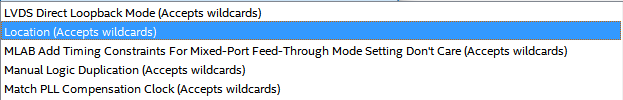
\includegraphics[scale=0.65]{figures/figure24.png}
   \caption{The available assignment names for a DE-series board.} 
	 \label{fig:24}
	 \end{center}
\end{figure}


\begin{figure}[H]
   \begin{center}
      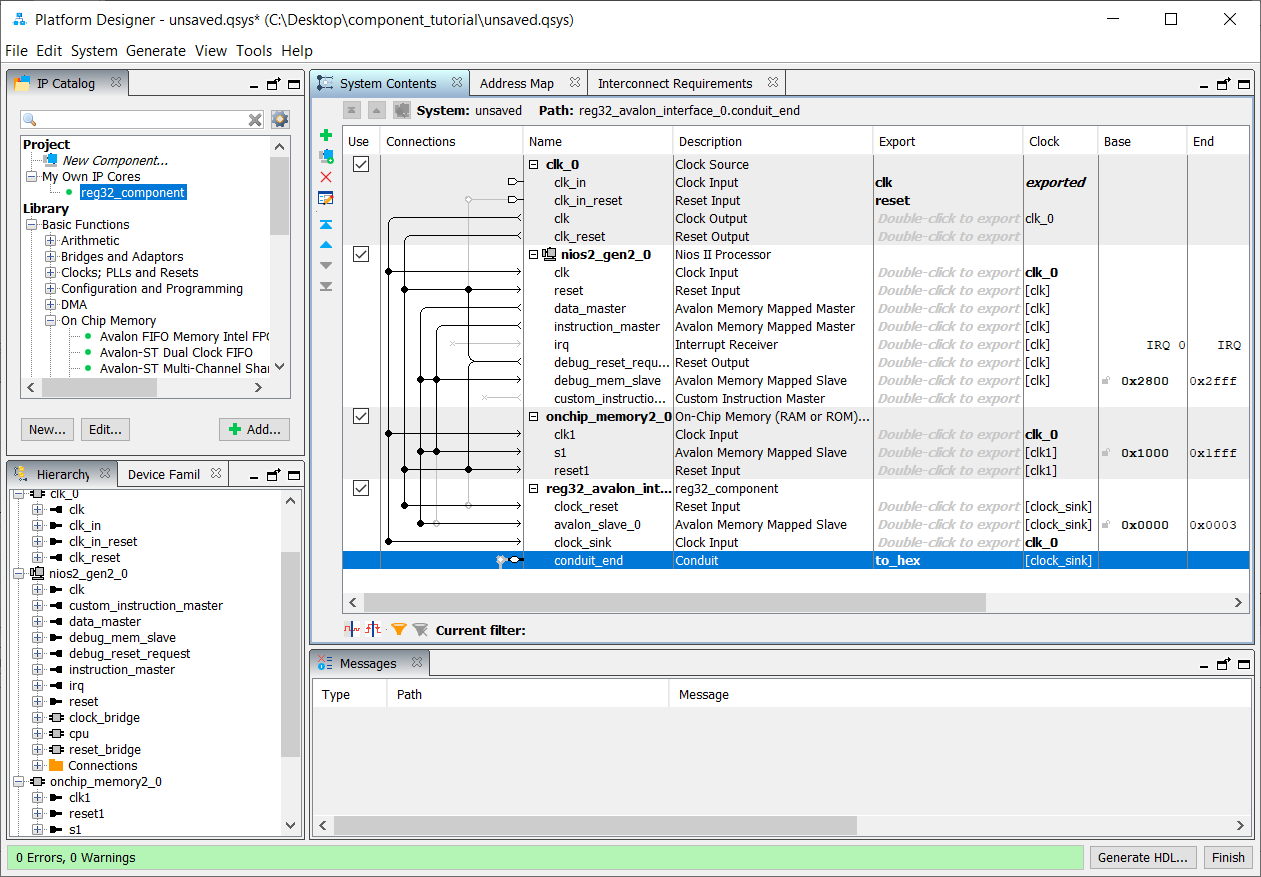
\includegraphics[scale=0.65]{figures/figure25.png}
   \caption{The complete assignment.} 
	 \label{fig:25}
	 \end{center}
\end{figure}

The DE-series board has fixed pin assignments. Having finished one design, the user will want
to use the same pin assignment for subsequent designs. Going through the procedure 
described above becomes tedious if there are many pins used in the design.
A useful Quartus Prime feature allows the user to both
export and import the pin assignments from a special file format, 
rather than creating them manually
using the Assignment Editor. A simple file format that can be used for this purpose
is the {\it Quartus Settings File (QSF)} format. The format for the file for our simple project (on a DE5a-Net board) is

\begin{center}
\begin{verbatim}
	set_location_assignment PIN_AY28 -to x1
	set_location_assignment PIN_AM27 -to x2
	set_location_assignment PIN_T11 -to f
\end{verbatim}
\end{center}

\noindent
By adding lines to the file, any number of pin assignments can be created.
Such {\it qsf} files can be imported into any design project.

If you created a pin assignment for a particular project, you can export it
for use in a different project. To see how this is done, open again the Assignment Editor
to reach the window in Figure~\ref{fig:25}. Select {\sf Assignments $>$ Export Assignment} which leads to the
window in Figure~\ref{fig:26}. Here, the file {\it light.qsf} is available for export.
Click on {\sf OK}.
If you now look in the directory, you will see that
the file {\it light.qsf} has been created.
 
\begin{figure}[H]
   \begin{center}
      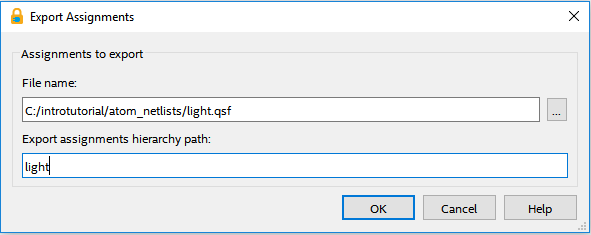
\includegraphics[scale=0.65]{figures/figure26.png}
   \caption{Exporting the pin assignment.} 
	 \label{fig:26}
	 \end{center}
\end{figure}

You can import a pin assignment by choosing {\sf Assignments $>$ Import Assignments}. 
This opens the dialogue in Figure~\ref{fig:27} to select the file to import. 
Type the name of the file, including the {\it qsf} extension and the full path
to the directory that holds the file, in the File Name box and press {\sf OK}.
Of course, you can also browse to find the desired file.
 
\begin{figure}[H]
   \begin{center}
      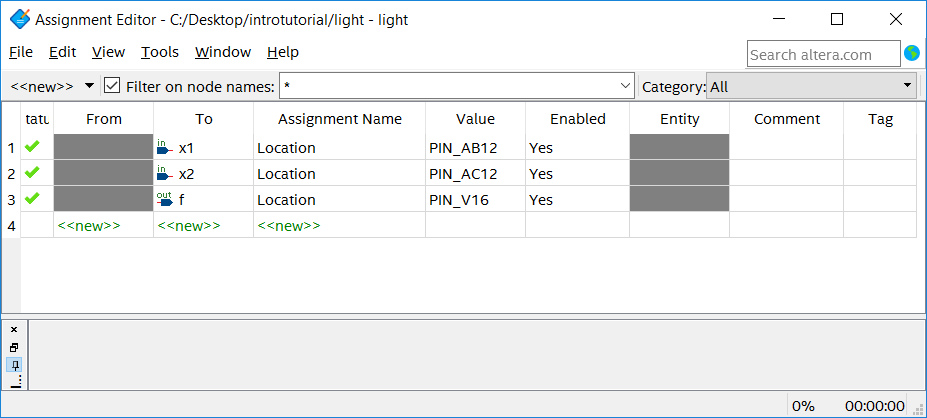
\includegraphics[scale=0.65]{figures/figure27.png}
   \caption{Importing the pin assignment.} 
	 \label{fig:27}
	 \end{center}
\end{figure}
